%!TEX TS-program = xelatex
%  Lab0.Rnw
%
%  Created by David Rosenberg on 2009-09-10.
%  Copyright (c) 2009 University of Chicago. All rights reserved.
%
\documentclass[10pt,letterpaper]{article}
\usepackage[Rpdflatex]{Rosenberg}
\usepackage{svn-multi}

\svnidlong
{$LastChangedDate: 2009-10-05 15:42:55 -0500 (Mon, 05 Oct 2009) $}
{$LastChangedRevision: 80 $}
{$LastChangedBy: root $}
% \svnid{$Id: example_main.tex 146 2008-12-03 13:29:19Z martin $}
% Don't forget to set the svn property 'svn:keywords' to
% 'HeadURL LastChangedDate LastChangedRevision LastChangedBy' or
% 'Id' or both depending if you use \svnidlong and/or \svnid
%
\newcommand{\svnfooter}{Last Changed Rev: \svnkw{LastChangedRevision}}
\svnRegisterAuthor{davidrosenberg}{David M. Rosenberg}


%\usepackage{Sweave}





\title{Introduction to computational programming\\\smaller Appendix 1\\\smaller Guide to Using \R}
\author{David M. Rosenberg\\\small University of Chicago\\\small Committee on Neurobiology\medskip\\
{\footnotesize \parbox[t]{10cm} {
Version control information:
\begin{tabbing}
\footnotesize\sffamily
 Last changes revision: \= \kill
 Last changed date: \> \svndate\\
 Last changes revision: \> \svnrev\\
 Version: \> \svnFullRevision*{\svnrev}\\
 Last changed by: \> \svnFullAuthor*{\svnauthor}\\
\end{tabbing}
}
}}

\begin{document}

\maketitle

\section{Overview}

This exercise is designed to serve as a practical introduction to the computational tools that will be used throughout this course.  It assumes no previous knowledge of numerical analysis nor experience in computer programming.

In order to help distinguish between \emph{code}, example output, computer commands and textual information, the following conventions will be used (both here and in later computational exercises).

\subsubsection{\emph{R} input}

Commands to be entered into the \emph{R} interpreter will be presented in \emph{syntax-highlighted} typewriter font, with the ``>'' character marking the beginning of each line.  Here is an example:

\begin{Schunk}
\begin{Sinput}
> 3 + 5
> help.start()
> load('myData.RData')
\end{Sinput}
\end{Schunk}

\subsubsection{\emph{R} output}

Output from the \emph{R} interpreter when shown, will be displayed directly after the corresponding input lines using the same font but in a different color and without the leading ``>''.

\begin{Schunk}
\begin{Sinput}
> 3 + 5
\end{Sinput}
\begin{Soutput}
[1] 8
\end{Soutput}
\begin{Sinput}
> randomData <- rnorm(n=100)
> summary(randomData)
\end{Sinput}
\begin{Soutput}
     Min.   1st Qu.    Median      Mean   3rd Qu.      Max. 
-2.805000 -0.683100  0.003494  0.033110  0.750600  2.992000 
\end{Soutput}
\end{Schunk}

\subsubsection{Computer commands / keyboard keys}

Following standard conventions, keyboard commands/shortcuts will be printed inline with the text in black typewriter font.  Combinations of keys which must be pressed simultaneously are separated by hyphens.  Keys to be pressed sequentially are separated by spaces.  ``Modifier keys'' (which vary in name from keyboard to keyboard) are denoted using a capital \texttt{C} or \texttt{M}.  Keyboard notation is summarized below:


\begin{itemize}
  \item \emph{Control:} Typically the ``control'' key abbreviated as \texttt{C-}
  \item \emph{Meta:} Usually the ``alt'' on standard keyboards and the ``command'' on apple keyboards, abbreviated as \texttt{M-}
  \item \emph{Enter:} Variously termed ``enter'', ``return'', ``carriage return'', ``linefeed'', and ``newline'', abbreviated as \texttt{[CR]}
  \item \emph{Directional arrows:} the arrow keys are represented by \texttt{[LEFT]}, \texttt{[RIGHT]}, \texttt{[UP]}, and \texttt{[DOWN]} respectively.
  \item \emph{Other keys:} Other keys are represented similarly, such as \texttt{[Esc]}, \texttt{[F1]} and \texttt{[TAB]}.
\end{itemize}


For example \texttt{C-c} means to simultaneously press the ``Control key'' and the letter ``c''.  \texttt{C-x C-c} means to first simultaneously press the ``Control'' key and the letter ``x'', then to simultaneously press the ``Control'' key and the letter ``c'', and \texttt{[Esc] : q !} means to sequentially press ``escape'', the ``colon'' (requires \texttt{[shift]}), ``q'' and the exclamation point (requires \texttt{[shift]}).


Make sure to pay special to similar looking characters such as
\begin{itemize}
  \item Single- (\textcolor{simpleRed}{\textbf{\'}}), double- (\textcolor{simpleRed}{\textbf{\"}}) and ``back-'' (\textcolor{simpleRed}{\textbf{\`}}) quotes
  \item Parentheses (\textcolor{simpleRed}{\textbf{ ( ) }}), brackets (\textcolor{simpleRed}{\textbf{ [ ] }}) and braces (\textcolor{simpleRed}{\textbf{ \{ \} }})
\end{itemize}

Graphical menus navigation is represented by placing boxes around menu and button names, such as \fbox{\texttt{File}} - \fbox{\texttt{Quit}}.

\subsection{Source text} % (fold)
\label{sub:source_text}

Large sections of source code and file contents will be displayed similarly to \R code with the following exceptions.
\begin{enumerate}
  \item The select will be surrounded by a box. 
  \item No prompts will be displayed (see section \ref{ssub:prompt} on page \pageref{ssub:prompt})
  \item A header comment (see section \ref{sub:style} on page \ref{sub:style}) will give the name of the file, URL to download it and other metadata
\end{enumerate}

Here is an example \R source file.

\begin{RBlistfloat}[h!]
\begin{Schunk}
\begin{Sinput}
 #!/usr/bin/env rr
 # encoding: utf-8
 # sumDigits.R
 #
 # sumDigits - a function which takes as input a number and returns the
 #            sum of its digits
 #
 # Example:
 #       > sumDigits(15)
 #       [1] 6
 #       > sumDigits(c(10, 122, 134))
 #       [1] 1 5 8
 #
 sumDigits <- function(x) {
   return(sum(as.integer(strsplit(as.character(x), '')[[1]])))
 }
\end{Sinput}
\end{Schunk}
\end{RBlistfloat}
%\end{quotation}
%\lstdefinestyle{Rinstyle}{style=RinstyleO,frame=none,keywordstyle={\bf\color{RRecomdcolor}},otherkeywords={!,!=,~,*,\&,\%/\%,\%*\%,\%\%,<-,<<-,/, \%in\%}}

% subsection source_text (end)
% section* Overview (end)
\part{Tutorial} % (fold)
\label{prt:tutorial}



\section{Getting Started}

While not strictly necessary, many students find it helpful to have access to \emph{R} and associated tools on their own computers.  Fortunately, \emph{R} is \emph{free software}\footnote{By calling \emph{R free software}, we are saying both that: \begin{enumerate} \item You don't have to pay to use \emph{R} (free as in beer) \item You are free to examine and improve \emph{R} as you like (free as in speech)\end{enumerate}.}, and available for most computing platforms.

\subsection{GNU \emph{R}}

The R homepage \url{http://r-project.org} provides compiled binaries for Windows, OS X, and linux platforms as well as the source distributions (for other platforms).  The following are platform specific installation instructions for the most common scenarios.

\subsubsection{Mac OSX} % (fold)
\label{ssub:mac_osx}

The Mac OSX binary distribution of \emph{R} can be downloaded from  \url{http://streaming.stat.iastate.edu/CRAN/bin/macosx/} as a \texttt{.dmg} file.  After downloading the image, simply open the \texttt{.dmg} file and drag the \texttt{R.app} icon into your \texttt{Applications} folder.

Once you have done this, starting \emph{R} is as easy as double-clicking the \texttt{R.app} icon in your \texttt{Applications} folder.  Alternatively, you may run \emph{R} in a console window by opening \texttt{Terminal.app} (located in the \texttt{Utilities} subfolder of \texttt{Applications}) and typing \texttt{R}\footnote{If you have trouble with this, it may be due to having the default \texttt{PATH} set incorrectly.  See me for details.}.

Running \texttt{R.app} provides you with some additional GUI functionality,
provided through the menu interface, such as a \emph{R} source editor
(\MenuC{File} - \MenuC{New Document}), a package manipulation and installation tool (\MenuC{Packages \& Data} - \MenuC{Package Installer}) and easy access to package guides (\MenuC{Help} - \MenuC{Vignettes}).

% subsubsection mac_osx (end)

\subsubsection{Windows} % (fold)
\label{ssub:windows}

Installing \emph{R} under windows is accomplished by downloading the windows binary installer from \url{http://streaming.stat.iastate.edu/CRAN/bin/windows/base/}, opening the installer and following the on-screen directions.  Upon completion of the installer (and possibly rebooting), you should have an icon labelled \texttt{R 2.9.2} on your desktop (and possibly in the \texttt{Start} menu as well).

To start a new \emph{R} session, simply double-click on the \texttt{R 2.9.2} icon.
% subsubsection windows (end)

\subsubsection{Linux} % (fold)
\label{ssub:linux}

Installing \emph{R} on a linux system can generally be performed using your distribution-specific package manager (\texttt{rpm/yum} for RedHat-type distributions, \texttt{apt} for Debian based distributions such as Ubuntu).

If your distribution does not provide \emph{R} packages, you can download the compressed sources from \url{http://streaming.stat.iastate.edu/CRAN/bin/linux/ubuntu/} and compile them yourself\footnote{If you need help with this, see me.}.


% \TODO{Dependency issues}
% TODO Linux dependency issues

% subsubsection linux (end)

\subsubsection{Other options} % (fold)
\label{ssub:other_options}

Should none of the above options prove successful for you, alternative methods of running \emph{R} do exist.  \R can be run remotely or, alternately, can be run inside of a java virtual machine.  If you need to consider any of these options, please see me.


% \begin{itemize}
%    \item Java i.e. Biocep
%    \item remote (ssh)
%\end{itemize}
% subsubsection other_options (end)

\subsection{Text Editor}

A \emph{Text editor} is a program that lets you edit \emph{plain text} documents (such as \emph{R} source code) without inserting any formatting or other markup (as you would find in a document edited by Microsoft Word.)  Additionally, all of the text editors described below provide additional capabilities to aid in the writing of \emph{R} source code.

At first glance, the use of a text editor may seem superfluous; why edit your code elsewhere instead of typing it directly into \emph{R}.  The answer to this is threefold:
\begin{enumerate}
  \item \textbf{Repeatability:} The act of typing code directly into an interpreter is innately error prone.  Additionally, you will often find ``chunks'' of code which you find yourself using over and over.  In order to speed up this process and ensure that the same code is used every time, it is beneficial to save the ``chunk'' in a code file.  A text editor is the proper tool for this.
  \item \textbf{Communication:} Having code stored in a text file makes it easy to share between users.
  \item \textbf{Analysis:} Having code stored in a text file enables easy post-hoc analysis and modification.
\end{enumerate}

With these benefits in mind, I recommend that each student find a text editor that they become comfortable with.  The following are some suggestions:

\subsubsection{Cross-platform} % (fold)
\label{ssub:cross_platform}

\emph{Cross-platform} tools are tools which are available on multiple operating systems (i.e. Mac OSX, Windows, etc).  Of the three cross-platform text editors listed below, two deserve special mention.  \emph{Vi(m)} and \emph{Emacs} are the two most popular text editors in the world.  They can be found on most modern operating systems without installing any software (with the exception of windows).  They are both very mature tools with a lot of features, but both carry a significant learning curve.  If you use Mac OSX or Linux, I would highly encourage you to take a look at one (or both) of them even if you don't end up using it as your ``primary'' text editing tool.

\begin{itemize}
    \item \textbf{vi(m)} is (arguably) easier to use and learn than \emph{Emacs}, and is available (as a source package) at  \url{ftp://ftp.vim.org/pub/vim/unix/vim-7.2.tar.bz2}.
    \item \textbf{Emacs}, though somewhat more difficult to get started with, is a more full-featured tool and has a special add-on package called \emph{ESS (Emacs Speaks Statistics)} which provides high-level integration with \emph{R}.
    \item \textbf{jedit} is a relatively new Java-based cross-platform editor which can be downloaded (all platforms) from  \url{http://prdownloads.sourceforge.net/jedit/jedit42install.jar}.
\end{itemize}
% subsubsection cross_platform (end)

\subsubsection{Mac OSX} % (fold)
\label{ssub:mac_osx2}

The following \emph{OS X} specific text-editors deserve special mention.

\begin{itemize}
    \item \textbf{TextMate}, available at \url{http://macromates.com/} is a very easy-to-use and powerful text editor that I \emph{highly} recommend to anyone running \emph{OS X}.
    \item \textbf{MacVim}, available at \url{http://code.google.com/p/macvim/} is an enhanced version of \emph{Vi(m)} which provides additional GUI capabilities and ease-of-use enhancements.
    \item \textbf{Aquamacs}, available at \url{http://aquamacs.org/} is an enhanced version of \emph{Emacs} which provides GUI integration, ease-of-use enahancements, and includes many add-on packages such as \emph{ESS}.
\end{itemize}
% subsubsection mac_osx2 (end)

\subsubsection{Windows} % (fold)
\label{ssub:windows2}

The default windows text editor, \emph{Notepad}, provides only the bare minimum of features.  Recommended alternatives include:

\begin{itemize}
    \item \textbf{Gvim}, available at \url{ftp://ftp.vim.org/pub/vim/pc/gvim72.exe}, provides the power of the \emph{vi} editor to windows users as well as an easier to use GUI.
    \item \textbf{Emacs} for windows can be downloaded from  \url{http://ftp.gnu.org/pub/gnu/emacs/windows/emacs-23.1-bin-i386.zip}.  I have no experience using \emph{emacs} under windows.
    \item \textbf{e-texteditor} is a \emph{TextMate} clone (see  \ref{ssub:mac_osx2}), providing many of the same features and the ability to use \emph{TextMate} extensions.  It is available from  \url{http://www.e-texteditor.com/}.
    \item \textbf{notepad++} is another popular Windows text-editor with which I have no experience.  It can be downloaded from  \url{http://notepad-plus.sourceforge.net/uk/site.htm}.
\end{itemize}
% subsubsection windows2 (end)

\section{Your first \emph{R} session}
\label{sec:first_r_session}

Lets dive right into your first \emph{R} session.  If you are in the lab, Click on the \texttt{Finder} icon, click \texttt{Applications} in the left sidebar, find the Open \texttt{R.app} icon, and double-click it.  You should be greeted by a message similar to

\begin{Schunk}
\begin{Soutput}
R version 2.10.0 Under development (unstable) (2009-06-03 r48708)
Copyright (C) 2009 The R Foundation for Statistical Computing
ISBN 3-900051-07-0

R is free software and comes with ABSOLUTELY NO WARRANTY.
You are welcome to redistribute it under certain conditions.
Type 'license()' or 'licence()' for distribution details.

  Natural language support but running in an English locale

R is a collaborative project with many contributors.
Type 'contributors()' for more information and
'citation()' on how to cite R or R packages in publications.

Type 'demo()' for some demos, 'help()' for on-line help, or
'help.start()' for an HTML browser interface to help.
Type 'q()' to quit R.

>
\end{Soutput}
\end{Schunk}

\subsection{Interpreter}

Try entering the following commands into the \emph{R} interpreter.

\begin{Schunk}
\begin{Sinput}
> 3
> 3 + 5
> 1:50
> x <- 1:5
> x / 2
\end{Sinput}
\end{Schunk}

You should see the following result:

\begin{Schunk}
\begin{Sinput}
> 3
\end{Sinput}
\begin{Soutput}
[1] 3
\end{Soutput}
\begin{Sinput}
> 3 + 5
\end{Sinput}
\begin{Soutput}
[1] 8
\end{Soutput}
\begin{Sinput}
> 1:50
\end{Sinput}
\begin{Soutput}
 [1]  1  2  3  4  5  6  7  8  9 10 11 12 13 14 15 16 17 18 19 20 21 22 23 24 25
[26] 26 27 28 29 30 31 32 33 34 35 36 37 38 39 40 41 42 43 44 45 46 47 48 49 50
\end{Soutput}
\begin{Sinput}
> x <- 1:50
> x / 2
\end{Sinput}
\begin{Soutput}
 [1]  0.5  1.0  1.5  2.0  2.5  3.0  3.5  4.0  4.5  5.0  5.5  6.0  6.5  7.0  7.5
[16]  8.0  8.5  9.0  9.5 10.0 10.5 11.0 11.5 12.0 12.5 13.0 13.5 14.0 14.5 15.0
[31] 15.5 16.0 16.5 17.0 17.5 18.0 18.5 19.0 19.5 20.0 20.5 21.0 21.5 22.0 22.5
[46] 23.0 23.5 24.0 24.5 25.0
\end{Soutput}
\end{Schunk}

Lets go through this one line at a time.

\begin{Schunk}
\begin{Sinput}
> 3
\end{Sinput}
\begin{Soutput}
[1] 3
\end{Soutput}
\end{Schunk}

The \emph{R} interpreter runs in what is called a \emph{Read-Evaluate-Print} loop.  It \emph{reads} in commands as you type them, \emph{evaluates} those commands, and finally \emph{prints} the result to the screen.  Here, you entered the number \texttt{3}, which was evaluated to \texttt{3}, and printed to the screen.  The \texttt{[1]} preceding the \texttt{3} in the output indicates that there is only one result.

\begin{Schunk}
\begin{Sinput}
> 3 + 5
\end{Sinput}
\begin{Soutput}
[1] 8
\end{Soutput}
\end{Schunk}

Here, the \emph{R} interpreter evaluated the expression \texttt{3 + 5} and printed the result, \texttt{8}.

\begin{Schunk}
\begin{Sinput}
> 1:50
\end{Sinput}
\begin{Soutput}
 [1]  1  2  3  4  5  6  7  8  9 10 11 12 13 14 15 16 17 18 19 20 21 22 23 24 25
[26] 26 27 28 29 30 31 32 33 34 35 36 37 38 39 40 41 42 43 44 45 46 47 48 49 50
\end{Soutput}
\end{Schunk}

This expression introduces an important concept in \emph{R}.  The expression \texttt{1:5} means (to \emph{R}) ``all whole numbers between 1 and 50, inclusive'' and represents a \emph{vector}\footnote{This will be elaborated on \ref{sub:ex_variables_intro} (page \pageref{sub:ex_variables_intro}).} or collection of values.  In order to display this result on the screen, the numbers from 1 to 50 are split over several lines.  Each line begins with a number in brackets, which denotes the ``number'' of each result.

\begin{Schunk}
\begin{Sinput}
> x <- 1:50
\end{Sinput}
\end{Schunk}

This expression introduces two additional important concepts.  The first is that of a \emph{variable}.  A \emph{variable} is a symbol which has a value assigned to it.  Here \texttt{x} is a variable.  The second concept is that of \emph{assignment}\footnote{If you have used other programming languages before, this may seem strange (traditionally, \texttt{=} was used for assignment).  Although \emph{R} will generally permit you to use \texttt{=} instead of \texttt{<-} for assignment, this practice is strongly discouraged.}.  It is the most basic of of variable operations, and is represented by the characters \texttt{<-}.  The assignment operator works by taking the expression to its right (\texttt{1:50}), and assigning it to the variable to its left (\texttt{x}).  From this point forward, typing \texttt{x} by itself is \emph{exactly} the same as typing \texttt{1:50}.  Try it.  enter the following:
\begin{Schunk}
\begin{Sinput}
> x
\end{Sinput}
\begin{Soutput}
 [1]  1  2  3  4  5  6  7  8  9 10 11 12 13 14 15 16 17 18 19 20 21 22 23 24 25
[26] 26 27 28 29 30 31 32 33 34 35 36 37 38 39 40 41 42 43 44 45 46 47 48 49 50
\end{Soutput}
\end{Schunk}
The result such be exactly the same as when you typed \texttt{1:50}.

\begin{Schunk}
\begin{Sinput}
> x / 2
\end{Sinput}
\begin{Soutput}
 [1]  0.5  1.0  1.5  2.0  2.5  3.0  3.5  4.0  4.5  5.0  5.5  6.0  6.5  7.0  7.5
[16]  8.0  8.5  9.0  9.5 10.0 10.5 11.0 11.5 12.0 12.5 13.0 13.5 14.0 14.5 15.0
[31] 15.5 16.0 16.5 17.0 17.5 18.0 18.5 19.0 19.5 20.0 20.5 21.0 21.5 22.0 22.5
[46] 23.0 23.5 24.0 24.5 25.0
\end{Soutput}
\end{Schunk}

Here we show that the variable \texttt{x} can be used just like a number, and that basic operations (such as division) operate on all elements of a vector.

\subsubsection{Example 1} % (fold)
\label{ssub:example_1}

Here is another example session for you to try, exploring further features of the \emph{R} interpreter.

\begin{Schunk}
\begin{Sinput}
> x <- rnorm(50, mean=4)
> x
\end{Sinput}
\begin{Soutput}
 [1] 4.847814 4.663077 3.972773 3.628680 5.051461 3.916160 4.106091 4.808384
 [9] 3.675945 4.497151 4.203201 2.873362 3.458051 4.375747 4.459771 4.067658
[17] 1.565833 4.268010 3.336798 4.603285 3.280433 3.396879 3.304621 2.946366
[25] 3.853675 3.801768 3.820183 4.145885 4.378447 4.512289 4.304202 4.385907
[33] 3.725495 2.799689 3.770407 4.113753 2.995331 1.832280 2.994591 4.811910
[41] 5.593934 4.950304 5.404499 3.266961 4.161115 3.874983 5.782598 5.431820
[49] 3.783462 2.471060
\end{Soutput}
\begin{Sinput}
> mean(x)
\end{Sinput}
\begin{Soutput}
[1] 3.965482
\end{Soutput}
\begin{Sinput}
> range(x)
\end{Sinput}
\begin{Soutput}
[1] 1.565833 5.782598
\end{Soutput}
\begin{Sinput}
> hist(x)
\end{Sinput}
\end{Schunk}
\begin{Schunk}
\begin{Sinput}
> ?hist
\end{Sinput}
\end{Schunk}
\begin{center}
\begin{Schunk}
\begin{Sinput}
> hist(x, main='my first plot', )
\end{Sinput}
\end{Schunk}
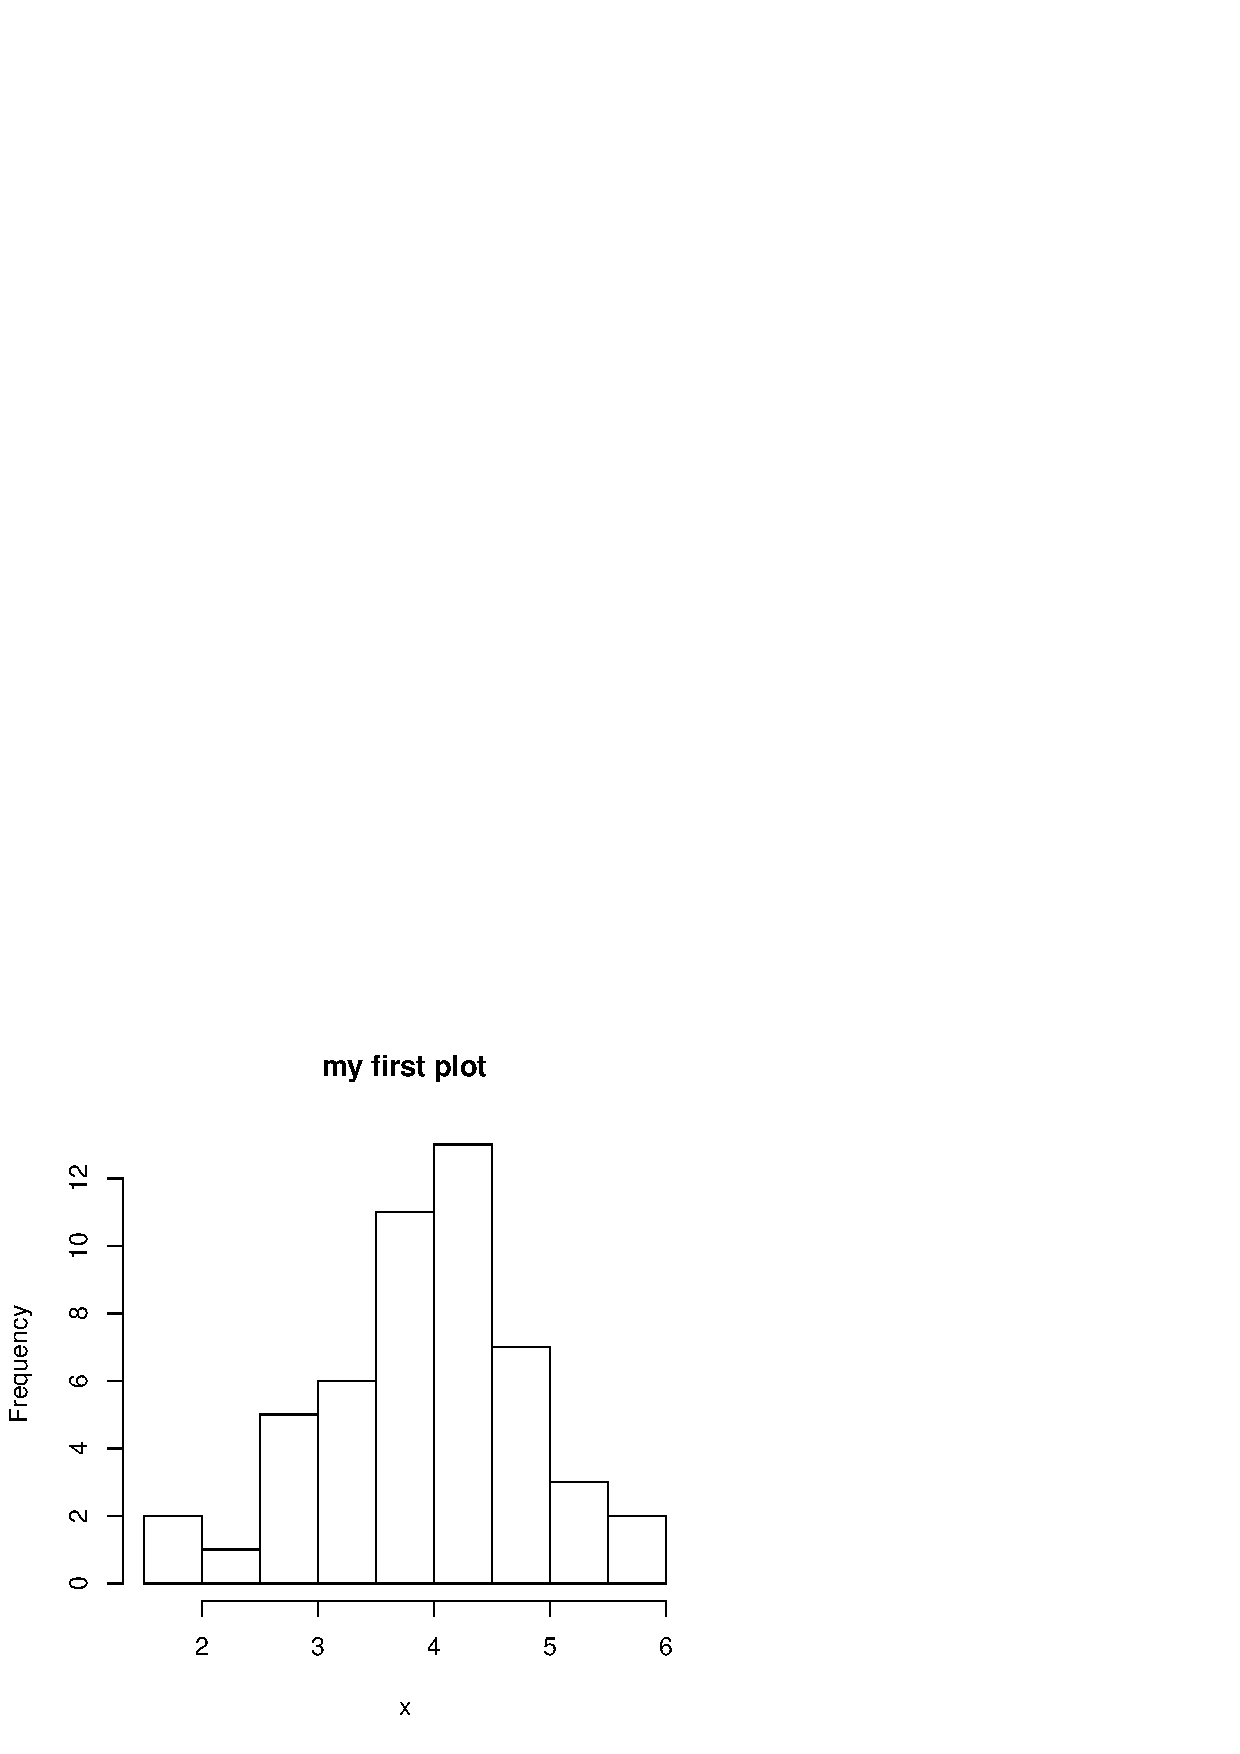
\includegraphics{guide_chapter0-firstsessionplot}
\end{center}

% subsubsection example_1 (end)

The \emph{R} interpreter includes several useful features.

\subsubsection{Tab completion} % (fold)
\label{ssub:tab_completion}


\emph{Tab completion} is a process where a partially entered command is completed by the interpreter by looking for any possible command containing the text you have typed.  Tab completion is performed by pressing the \texttt{[TAB]} key after typing part of a command.  Try it.  Suppose you couldn't remember the name of the command for finding square roots.  Type into the interpreter \texttt{sq} and, without typing anything else, press the \texttt{[TAB]} key.  You should find that \texttt{sq} has been expanded to \texttt{sqrt}!  If there is more than one possible completion for the text you have entered, tab-completion will list all possible completions if you press \texttt{[TAB]} twice.  Try getting all completions of \texttt{exp}.  The result should look something like this\footnote{In the OSX GUI, a pop-up menu showing possible completions will be shown instead of printing the possibilities to the screen.}.

\begin{Schunk}
\begin{Sinput}
> exp
\end{Sinput}
\end{Schunk}
\begin{Schunk}
\begin{Soutput}
exp
exp	expand.grid	expand.model.frame	expm1	expression
\end{Soutput}
\end{Schunk}

Tab-completion can also be used to find the arguments to a function.  Consider the \texttt{plot} function.  It has far too many options to remember.  But, but typing \texttt{plot(} and pressing the \texttt{[TAB]} key, \emph{R} will show you all possible arguments to the function \texttt{plot}\footnote{In the OSX GUI, tab-completion for function arguments does not work.  Instead, the syntax for the function (including arguments) is always shown along the bottom of the GUI window.}.

\begin{Schunk}
\begin{Soutput}
> plot(
\end{Soutput}
\end{Schunk}
\begin{Schunk}
\begin{Soutput}
  [1] ""                  "...="              "ci.lty="          
  [4] "do.points="        "log="              "panel.last="      
  [7] "x="                "absVal="           "ci.type="         
 [10] "edge.root="        "lty.intervals="    "panel="           
 [13] "xaxt="             "add.smooth="       "ci="              
 [16] "edgePar="          "lty.predicted="    "par.fit="         
 [19] "xlab="             "add="              "col.01line="      
 [22] "formula="          "lty.separator="    "pch="             
 [25] "xlim="             "angle="            "col.hor="         
 [28] "frame.plot="       "lty="              "plot.type="       
 [31] "xpd="              "ann="              "col.intervals="   
 [34] "freq="             "lwd="              "predicted.values="
 [37] "xval="             "ask="              "col.points="      
 [40] "grid="             "main2="            "qqline="          
 [43] "xy.labels="        "asp="              "col.predicted="   
 [46] "hang="             "main="             "range.bars="      
 [49] "xy.lines="         "axes="             "col.range="       
 [52] "horiz="            "mar.multi="        "separator="       
 [55] "y="                "border="           "col.separator="   
 [58] "id.n="             "mar="              "set.pars="        
 [61] "yax.flip="         "caption="          "col.vert="        
 [64] "intervals="        "max.mfrow="        "sub.caption="     
 [67] "yaxt="             "center="           "col="             
 [70] "label.pos="        "mgp="              "sub="             
 [73] "ylab="             "cex.caption="      "conf="            
 [76] "labels.id="        "nc="               "subset="          
 [79] "ylim="             "cex.id="           "cook.levels="     
 [82] "labels="           "nodePar="          "type="            
 [85] "zero.line="        "cex.main="         "dLeaf="           
 [88] "leaflab="          "oma.multi="        "verbose="         
 [91] "cex.points="       "data="             "legend.text="     
 [94] "oma="              "verticals="        "ci.col="          
 [97] "density="          "levels="           "panel.first="     
[100] "which="           
\end{Soutput}
\end{Schunk}

Finally, tab-completion can be used to complete filenames when used inside single or double quotation marks.

% subsubsection tab_completion (end)

\subsubsection{History} % (fold)
\label{ssub:history}

A second useful feature of the \emph{R} interpreter is the \emph{command history}.  \emph{R} keeps a record of every command you have entered since opening the \emph{R} interpreter.  At the \texttt{>} prompt, you can use the \texttt{[UP]} and \texttt{[DOWN]} arrows to move backwards and forwards through your command history.  Try it.

You can view your full command history by using the command \texttt{history()} (press texttt{q} to quit the history browser).  Finally, you can use the command \texttt{savehistory()} to write your history to a text file for later inspection (default name is \texttt{.Rhistory}).

% subsubsection history (end)

\subsubsection{Comments} % (fold)
\label{ssub:comments}

In \emph{R}, the pound character (\texttt{\#}) is used to denote comments.  In general anything after between a \texttt{\#} and the end of a line is ignored.  This allows explanations and textual notes to be included directly in \emph{R} source code.  The only time that a \texttt{\#} does not indicate a comment is when it is surrounded by single- or double- quotation marks.

\begin{Schunk}
\begin{Sinput}
> # This is a comment
> '# This is not a comment'
\end{Sinput}
\begin{Soutput}
[1] "# This is not a comment"
\end{Soutput}
\end{Schunk}

% subsubsection comments (end)

\subsubsection{Prompt} % (fold)
\label{ssub:prompt}

As you have seen, the standard \emph{R} prompt is the \texttt{>} character.  Occasionally, you will see the plus sign (\texttt{+}) shown as a prompt instead.  This is a \emph{continuation prompt} and signifies that the command entered on the previous line is not complete.  This allows you to break long commands over multiple lines.

\begin{Schunk}
\begin{Sinput}
> 3 + 5 +
+ 2
\end{Sinput}
\begin{Soutput}
[1] 10
\end{Soutput}
\begin{Sinput}
> sqrt(
+   3.141)
\end{Sinput}
\begin{Soutput}
[1] 1.772287
\end{Soutput}
\end{Schunk}

Occasionally, other (self-explanatory) prompts will be shown, such as
\begin{Schunk}
\begin{Soutput}
Hit <Return> to see the next plot: 
\end{Soutput}
\end{Schunk}
% subsubsection prompt (end)

\subsubsection{Exploring the current environment} % (fold)
\label{ssub:exploring_the_current_environment}

Sometimes, it is easy to loose track of the variables you have defined.  \R provides a simple command to view them: \Com{ls()}.

\begin{Schunk}
\begin{Sinput}
> ls()
\end{Sinput}
\begin{Soutput}
[1] "oldRout"         "oldRset"         "plotCompletions" "randomData"     
[5] "startuptext"     "x"              
\end{Soutput}
\begin{Sinput}
> ls(all.names=TRUE)
\end{Sinput}
\begin{Soutput}
 [1] ".myRset"         ".Random.seed"    ".required"       ".Rout"          
 [5] "oldRout"         "oldRset"         "plotCompletions" "randomData"     
 [9] "startuptext"     "x"              
\end{Soutput}
\end{Schunk}
% subsubsection exploring_the_current_environment (end)


\subsubsection{Getting help}

One of \R \'s greatest strengths is the availability of online help inside the interpreter.  When inside the \R help system, you can move up and down with the arrow keys, and return to the interpreter by pressing \texttt{q}.

\subsubsection{Help browser} % (fold)

There are two general ways to invoke the \R help system (described below).

\begin{itemize}
  \item Using the \texttt{help} command:
\end{itemize}

\begin{Schunk}
\begin{Sinput}
> help('plot')
\end{Sinput}
\end{Schunk}
\begin{Schunk}
\begin{Soutput}
plot                package:graphics                R Documentation

Generic X-Y Plotting

Description:

     Generic function for plotting of R objects.  For more details
     about the graphical parameter arguments, see 'par'.

Usage:
\end{Soutput}
\end{Schunk}

\begin{itemize}
  \item Using the \texttt{?} shortcut:
\end{itemize}

\begin{Schunk}
\begin{Sinput}
> ?plot
\end{Sinput}
\end{Schunk}
% <<help_ex2_1,eval=t,echo=f>>=
% plot_help <- help('plot')
% plot_help_text <- paste(readLines(plot_help), collapse="\n");
% plot_help_text <- gsub('_\\\b(.{1})', '\\1', plot_help_text);
% cat(plot_help_text);
% @
%
In general, you can receive help for any command \emph{\texttt{thisCommand}} using either \texttt{help('\emph{thisCommand}')}\footnote{Note the use of quotation marks.} or with \texttt{?\emph{thisCommand}}.

In increase the scope of your search of the help system, try

\begin{Schunk}
\begin{Sinput}
> help.search('plot')
> ??plot
\end{Sinput}
\end{Schunk}

Finally, you can invoke the \emph{HTML} help browser (if available) using the command \texttt{help.start()}.

% subsubsection help_browser (end)

\subsubsection{Examples} % (fold)
\label{ssub:examples}

Another feature of the online help systems is the \Com{example()} function.  \R will print and execute any code shown in the ``Examples'' section of a command\'s online help.

\begin{Schunk}
\begin{Sinput}
> example('Arithmetic')
\end{Sinput}
\begin{Soutput}
Arthmt> x <- -1:12

Arthmt> x + 1
 [1]  0  1  2  3  4  5  6  7  8  9 10 11 12 13

Arthmt> 2 * x + 3
 [1]  1  3  5  7  9 11 13 15 17 19 21 23 25 27

Arthmt> x %% 2 #-- is periodic
 [1] 1 0 1 0 1 0 1 0 1 0 1 0 1 0

Arthmt> x %/% 5
 [1] -1  0  0  0  0  0  1  1  1  1  1  2  2  2
\end{Soutput}
\end{Schunk}

% subsubsection examples (end)


\subsubsection{Session} % (fold)
\label{ssub:session}

An \R session consists of the commands and variables created from the time you start the \R interpreter until you quit.  \R provides several facilities for managing, saving, and restoring sessions.

\begin{itemize}
    \item \texttt{save.image()} - This command saves the current session to a file named \Com{.RData} in the current directory.
    \item \texttt{save()} - This command saves an \R object (given as an argument) to a file.
    \item \texttt{load()} - This command takes as an argument a file (such as \Com{.RData}) and restores it into the current session.
    \item \Com{source()} - This command executes all \R commands in the file given as an argument.
    \item \texttt{dump()} - This command ``dumps'' the current session as a series of commands to a file given as an argument.  The file produced by \Com{dump()} make be loaded using \Com{source()}.
\end{itemize}

% subsubsection saving (end)

\subsubsection{Quitting} % (fold)
\label{ssub:quitting}

To quit the \R interpreter, use the command \Com{q()}.  \R will then ask you if you want to save the current session.  If you do, \Com{save.image()} will be used to write the current session to disk.

Note that, by default, \R \emph{always} loads the file \Com{.RData} on startup if it finds one in its working directory.  This means that \R will always load the most recently save session image.  To remove this file (within \R), you may issue the command \Com{unlink('.RData')}.

To clear the current session, issue the command \Com{rm(list=ls())}.

% subsubsection quitting (end)

\subsubsection{Aborting} % (fold)
\label{ssub:aborting}

Occasionally, you may find that \R seems ``stuck.''  Perhaps you mistakenly created an infinite loop or entered a prohibitively complicated command.  If you would like to cancel in in-progress computation, press \Com{C-c} to abort the running computation\footnote{In the OSX GUI, the \texttt{[Esc]} key is used instead}.  You can also use \Com{C-c} to clear a partially entered command and start at a clean \Com{>} prompt.  In the event this doesn't work, the operating system process manager can be used to halt the offending process\footnote{How this is done is operating system dependent.  In windows, \Com{C}-\Com{M}-\Com{[del]} will bring up the Task Manager, which may be used to terminate \R.  In Linux/MacOSX, the command \Com{sudo killall -9 \{R,R.app\}}, entered at a Terminal prompt will terminate \R.} 

% subsubsection aborting (end)

% subsection session (end)

\section{Exploring \emph{R}} % (fold)
\label{sec:exploring_r}

\subsection{Example 2: Calculator} % (fold)
\label{sub:example_2_calculator}

Included below are a couple of quick examples highlighting the use of \R as a calculator.  A more complete listing of basic calculation functions is provided in table~\ref{tab:arith_table} (page \pageref{tab:arith_table}).


\begin{table}[htbp]
  \bc
  \begin{tabular}{cp{6cm}}
    \toprule
    category & functions \\
    \midrule
    arithmetic & \texttt{+,-,*,/,\%\%} \\
    exponential & \texttt{exp(), log(), log10(), log2()} \\
    trigonometric & \texttt{cos(), sin(), tan(), acos(),asin(),atan() cosh(), sinh(), tanh(), acosh(), asinh(), atanh()} \\
    approximation & \texttt{abs(), sign(), sqrt(), floor(), ceiling(), trunc(), round(), signif()} \\
    \bottomrule
  \end{tabular}
  \ec
  \caption{\label{tab:arith_table}Table of standard mathematical functions}
\end{table}


\begin{Schunk}
\begin{Sinput}
> # Arithmetic
> 3 / 5
\end{Sinput}
\begin{Soutput}
[1] 0.6
\end{Soutput}
\begin{Sinput}
> 301 + 50000003
\end{Sinput}
\begin{Soutput}
[1] 50000304
\end{Soutput}
\begin{Sinput}
> 0.0005 * 0.0001
\end{Sinput}
\begin{Soutput}
[1] 5e-08
\end{Soutput}
\begin{Sinput}
> -0.0001 ** 9
\end{Sinput}
\begin{Soutput}
[1] -1e-36
\end{Soutput}
\begin{Sinput}
> -0.0001 ^ 9
\end{Sinput}
\begin{Soutput}
[1] -1e-36
\end{Soutput}
\begin{Sinput}
> ## exponentiation can be represented with either ** or ^
> 3 + 5 * 2
\end{Sinput}
\begin{Soutput}
[1] 13
\end{Soutput}
\begin{Sinput}
> (3 + 5) * 2
\end{Sinput}
\begin{Soutput}
[1] 16
\end{Soutput}
\begin{Sinput}
> ## special operations are called by name
> sin(3)
\end{Sinput}
\begin{Soutput}
[1] 0.14112
\end{Soutput}
\begin{Sinput}
> sqrt(5)
\end{Sinput}
\begin{Soutput}
[1] 2.236068
\end{Soutput}
\begin{Sinput}
> ## complex numbers are supported when written as x + yi
> -1 + 0i
\end{Sinput}
\begin{Soutput}
[1] -1+0i
\end{Soutput}
\begin{Sinput}
> sqrt(-1 + 0i)
\end{Sinput}
\begin{Soutput}
[1] 0+1i
\end{Soutput}
\begin{Sinput}
> ## constants can be called by name or expression (varies)
> pi
\end{Sinput}
\begin{Soutput}
[1] 3.141593
\end{Soutput}
\begin{Sinput}
> exp(1)
\end{Sinput}
\begin{Soutput}
[1] 2.718282
\end{Soutput}
\end{Schunk}
% subsection example_2_calculator (end)



\subsection{Example 3: Variables} % (fold)
\label{sub:ex_variables_intro}

As discussed in \ref{sec:first_r_session} (page \pageref{sec:first_r_session}), variables play a key part in computational programming.  In \R, variables are defined using the \cc{variable <- value} syntax.  Here, we will discuss some of the nuances and common pitfalls encountered when using variables in \R.

\subsubsection{Names} % (fold)
\label{ssub:vars_names}

Variable names in \R consist of letters, numbers, underscores, and periods (``.''), subject to the following constraints.
\begin{itemize}
  \item Variable names cannot start with an underscore or a number.  Variable names \emph{generally} should not begin with a period\footnote{Variables with names beginning with a period are ``hidden'' from the you and many of \R\'s internal functions. }.
  \item Variable names are case sensitive.  This means that the names \Com{myVariable} and \Com{myvariable} are \emph{not} the same.
  \item There are a small number of reserved variable names (listed in table \ref{tab:reserved_names}) which cannot be used.  In general, however, the names of \R functions are \emph{not} protected.  Thus, it is possible to define a variable named \Com{print} which will prevent you from using the \Com{print()} function.  Beware of this.
\end{itemize}

\begin{table}[htbp]
  \begin{center}
    \begin{tabular}{cccc}
      \toprule
      \multicolumn{4}{c}{\textnormal{Reserved Names}} \\
      \midrule\tt
      if & TRUE & else & FALSE \\
      repeat & NULL & while & Inf \\
      function & NaN & for & NA \\
      in & NA\_integer\_ & next & NA\_real\_ \\
      break & NA\_complex\_ \\
      \bottomrule
    \end{tabular}
    \caption{\label{tab:reserved_names}Reserved names in \R.}
  \end{center}
\end{table}

In addition to these restrictions, style\footnote{For more information on style, see \ref{sub:style}, page \pageref{sub:style}}. provides an additional list of \emph{suggestions}.

\begin{itemize}
  \item Variable names should be descriptive.  For example a variable containing the number of students in a class:  \Com{numStudents} - good, \Com{ns} - bad.
  \item Variable names should not be written in all capital letters and should not start with capital letters.  \Com{numStudents} - good, \Com{NUM\_STUDENTS} - bad, \Com{num\_students} - good, \Com{numstudents} - less good
\end{itemize}

% subsubsection names (end)

\subsubsection{Types} % (fold)
\label{subs:v_types}

Variables are classified by \emph{type}, that is, what ``kind'' of information they contain.  Just as names tell you ``who'' a variable is, types tell ``what'' a variable is.  In \R there a number of different \emph{types} suited for the analysis of different problems.  Here we shall explore only the most universal of \emph{types} provided in \R.  The basic \emph{types} are summarized in table \ref{tab:type_table}.

\begin{table}[htbp]
  \bc
  \begin{tabular}{cp{3.5cm}p{8cm}}
    \toprule
    type name & description & example \& usage notes \\
    \midrule
    numeric & number values & \texttt{3, 5, pi, 0.001, 10e6, 0+3i} \\
    logical & boolean values & \texttt{TRUE, FALSE} \\
    character & sequence of letters, numbers and punctuation & \texttt{"David Rosenberg", "MyCharacterString"} \emph{NOTE:} data of type character must be surrounded by either single or double quotation marks. \\
    function & a built-in or user defined function & \texttt{exp, print, help}\\
    \bottomrule
  \end{tabular}
  \caption{\label{tab:type_table}Basic data types}
  \ec
\end{table}


% subsubsection types (end)

\subsubsection{Attributes and coercion} % (fold)
\label{ssub:attributes_and_coercion}

It is possible (and sometimes necessary) to treat variables of one type as if they were of another type.  The process of converting data from one type to another is called \emph{coercion}, and is used most frequently when importing data from other programs (such as Microsoft Excel) into \R.  There are a set of commands in \R for performing variable coercion with names such as \Com{as.numeric()} and \Com{as.character()}.  If you need to use these functions, consult the online documentation for guidance.

One special case of coercion that does not require any commands is coercion from type \emph{numeric} to \emph{logical}.  A numeric variable equal to $0$ is treated as \Com{FALSE} when used as a logical.  All other numeric variables are treated as \Com{TRUE}.

%\TODO{Do attributes deserve mention here?}

% subsubsection attributes_and_coercion (end)

\subsubsection{Vectors and Matrices} % (fold)
\label{ssub:vectors}

It is often useful to use several ``values'' to describe a single ``thing'' or to refer to a group of related variables with a single name.  \R provides three constructs for creating multi-valued variables (all of which must be of the same type).

\textbf{Vectors} are the most basic of these ``compound'' variables and are, in fact, the primary way in which \R handles data.  Individual values in a vector (sometimes called members) are each assigned a unique integer or index.  The easiest way to think of a vector is as an ordered sequence.

\begin{displaymath}
  (a_n) = a_1, a2, \ldots
\end{displaymath}

Individual members of a vector are referenced by using brackets as follows

\begin{Schunk}
\begin{Sinput}
> firstVector <- letters[1:10];
> firstVector   # if no index is given, a variable name referes to all members
\end{Sinput}
\begin{Soutput}
 [1] "a" "b" "c" "d" "e" "f" "g" "h" "i" "j"
\end{Soutput}
\begin{Sinput}
> firstVector[5]    # The fifth member of firstVector
\end{Sinput}
\begin{Soutput}
[1] "e"
\end{Soutput}
\begin{Sinput}
> firstVector[5] <- 'E';  # Members can be assigned by indexing as well
> firstVector
\end{Sinput}
\begin{Soutput}
 [1] "a" "b" "c" "d" "E" "f" "g" "h" "i" "j"
\end{Soutput}
\end{Schunk}

Vectors are typically constructed using either the \Com{c()} command or using a special \Com{start:end} notation.
\begin{Schunk}
\begin{Sinput}
> secondVector <- c(1,4,9,16)         # c() is used to make vectors
> secondVector                        #
\end{Sinput}
\begin{Soutput}
[1]  1  4  9 16
\end{Soutput}
\begin{Sinput}
> biggerVector <- c(secondVector, 25) # and to add to them
> numVector <- 1:5                    # a vector of integers can by made using
> numVector                           #       the start:end notation
\end{Sinput}
\begin{Soutput}
[1] 1 2 3 4 5
\end{Soutput}
\begin{Sinput}
> numVector[c(1,3,5)]                 # You can use vectors to index vectors
\end{Sinput}
\begin{Soutput}
[1] 1 3 5
\end{Soutput}
\end{Schunk}

In general, most functions operations accept vectors just like regular variables and work in an element-wise fashion.  Exceptions to this rule include functions that only make sense with multi-valued input (such as \Com{max()}) and some user-generated functions.
\begin{Schunk}
\begin{Sinput}
> firstVector <- 1:15
> firstVector.1 <- firstVector / pi
> firstVector.1
\end{Sinput}
\begin{Soutput}
 [1] 0.3183099 0.6366198 0.9549297 1.2732395 1.5915494 1.9098593 2.2281692
 [8] 2.5464791 2.8647890 3.1830989 3.5014087 3.8197186 4.1380285 4.4563384
[15] 4.7746483
\end{Soutput}
\begin{Sinput}
> firstVector.2 <- sin(firstVector.1)
> firstVector.2
\end{Sinput}
\begin{Soutput}
 [1]  0.31296180  0.59448077  0.81627311  0.95605566  0.99978466  0.94306673
 [7]  0.79160024  0.56060280  0.27328240 -0.04149429 -0.35210211 -0.62733473
[13] -0.83953993 -0.96739776 -0.99806251
\end{Soutput}
\begin{Sinput}
> length(firstVector)           # length() is used to find out how many members
\end{Sinput}
\begin{Soutput}
[1] 15
\end{Soutput}
\begin{Sinput}
>                               # a vector has
> max(firstVector)              # largest member
\end{Sinput}
\begin{Soutput}
[1] 15
\end{Soutput}
\begin{Sinput}
> sum(firstVector)              # sum of all members
\end{Sinput}
\begin{Soutput}
[1] 120
\end{Soutput}
\begin{Sinput}
> firstVector > pi/2            # a logical vector is returned
\end{Sinput}
\begin{Soutput}
 [1] FALSE  TRUE  TRUE  TRUE  TRUE  TRUE  TRUE  TRUE  TRUE  TRUE  TRUE  TRUE
[13]  TRUE  TRUE  TRUE
\end{Soutput}
\end{Schunk}

\textbf{Matrices} are similar to vectors except that they have an additional dimension of indexing.  Matrices are generated with the \Com{matrix()} function and can be merged using the commands \Com{rbind()} and \Com{cbind()}.  Two important points about matrices to remember are:
\begin{enumerate}
  \item \R defaults to \emph{column-major} format for matrices\footnote{\emph{Column-major} format means that a it fills \emph{down} rows first, then across columns.}
  \item Arithmetic operations are normally performed elementwise on matrices.  Matrix multiplication and division are performed using \Com{\%*\%} and \Com{\%/\%}
\end{enumerate}

\begin{Schunk}
\begin{Sinput}
> matrix(data=c(1:12), nrow=4, ncol=3)    # Note how the values go DOWN first
\end{Sinput}
\begin{Soutput}
     [,1] [,2] [,3]
[1,]    1    5    9
[2,]    2    6   10
[3,]    3    7   11
[4,]    4    8   12
\end{Soutput}
\begin{Sinput}
> matrix(data=c(1:12), nrow=4, ncol=3, byrow=TRUE)   # byrow=TRUE avoids this
\end{Sinput}
\begin{Soutput}
     [,1] [,2] [,3]
[1,]    1    2    3
[2,]    4    5    6
[3,]    7    8    9
[4,]   10   11   12
\end{Soutput}
\begin{Sinput}
> matrix(c(1:12), 4, 3, byrow=TRUE)       # The xxx= are optional
\end{Sinput}
\begin{Soutput}
     [,1] [,2] [,3]
[1,]    1    2    3
[2,]    4    5    6
[3,]    7    8    9
[4,]   10   11   12
\end{Soutput}
\begin{Sinput}
> matrix(c(1:12), 4, byrow=TRUE)          # only one of nrow, ncol is needed
\end{Sinput}
\begin{Soutput}
     [,1] [,2] [,3]
[1,]    1    2    3
[2,]    4    5    6
[3,]    7    8    9
[4,]   10   11   12
\end{Soutput}
\begin{Sinput}
> matrix(c(1:12), ncol=3, byrow=TRUE)
\end{Sinput}
\begin{Soutput}
     [,1] [,2] [,3]
[1,]    1    2    3
[2,]    4    5    6
[3,]    7    8    9
[4,]   10   11   12
\end{Soutput}
\begin{Sinput}
> myMatrix <- matrix(c(1:12), 4, byrow=TRUE)
> t(myMatrix)                             # t() transposes a matrix
\end{Sinput}
\begin{Soutput}
     [,1] [,2] [,3] [,4]
[1,]    1    4    7   10
[2,]    2    5    8   11
[3,]    3    6    9   12
\end{Soutput}
\begin{Sinput}
> myMatrix
\end{Sinput}
\begin{Soutput}
     [,1] [,2] [,3]
[1,]    1    2    3
[2,]    4    5    6
[3,]    7    8    9
[4,]   10   11   12
\end{Soutput}
\begin{Sinput}
> myMatrix[4,3]                   # members are referenced by two indices
\end{Sinput}
\begin{Soutput}
[1] 12
\end{Soutput}
\begin{Sinput}
> myMatrix[4,]             # rows/columns are extracted by omitting an index
\end{Sinput}
\begin{Soutput}
[1] 10 11 12
\end{Soutput}
\begin{Sinput}
> myMatrix[,3]
\end{Sinput}
\begin{Soutput}
[1]  3  6  9 12
\end{Soutput}
\begin{Sinput}
> myMatrix[c(1:2), c(1:3)] # vector indexing works as before
\end{Sinput}
\begin{Soutput}
     [,1] [,2] [,3]
[1,]    1    2    3
[2,]    4    5    6
\end{Soutput}
\begin{Sinput}
> rbind(myMatrix, myMatrix)       # rbind() joins matrices vertically
\end{Sinput}
\begin{Soutput}
     [,1] [,2] [,3]
[1,]    1    2    3
[2,]    4    5    6
[3,]    7    8    9
[4,]   10   11   12
[5,]    1    2    3
[6,]    4    5    6
[7,]    7    8    9
[8,]   10   11   12
\end{Soutput}
\begin{Sinput}
> cbind(myMatrix, myMatrix)       # cbind() joins matrices horizontally
\end{Sinput}
\begin{Soutput}
     [,1] [,2] [,3] [,4] [,5] [,6]
[1,]    1    2    3    1    2    3
[2,]    4    5    6    4    5    6
[3,]    7    8    9    7    8    9
[4,]   10   11   12   10   11   12
\end{Soutput}
\begin{Sinput}
> myMatrix / 5                    # Operations are always performed element-wise
\end{Sinput}
\begin{Soutput}
     [,1] [,2] [,3]
[1,]  0.2  0.4  0.6
[2,]  0.8  1.0  1.2
[3,]  1.4  1.6  1.8
[4,]  2.0  2.2  2.4
\end{Soutput}
\begin{Sinput}
> myMatrix * myMatrix             # (Even multiplication)
\end{Sinput}
\begin{Soutput}
     [,1] [,2] [,3]
[1,]    1    4    9
[2,]   16   25   36
[3,]   49   64   81
[4,]  100  121  144
\end{Soutput}
\begin{Sinput}
> myMatrix %*% t(myMatrix)        # unless the %*% notation is used
\end{Sinput}
\begin{Soutput}
     [,1] [,2] [,3] [,4]
[1,]   14   32   50   68
[2,]   32   77  122  167
[3,]   50  122  194  266
[4,]   68  167  266  365
\end{Soutput}
\end{Schunk}

% subsubection vectors (end))

\textbf{Arrays} are similar to matrices and vectors except that they allow any number of dimensions.

\subsubsection{Lists and data.frames} % (fold)
\label{ssub:lists_and_data_frames}

There are two additional ``special'' data types in \R that you will encounter in this course.  Both might be considered generalizations of the data types discussed above.

\emph{Lists} (\cc{list()}) are a generalized form of the \cc{vector} data type.  They are a collection of ``values'', each of which is assigned an index.  The most important difference between lists and vectors is that lists can contain members of \emph{any} type\footnote{This includes other lists!  In fact, complex data structures are generally described using nested lists}.  Lists also use a slightly different syntax for member access, shown in Table~\ref{tab:list_syntax} (page \pageref{tab:list_syntax}).

\emph{Data frames} (\cc{data.frame()}) are a lot like matrices and arrays.  Unlike matrices and arrays, however, data frames allow different types for different \emph{columns} (although a single column must be of uniform type) and introduce an additional set of constraints.  Data frames \emph{always} have uniquely named rows and columns\footnote{Don't worry about these names just yet.  \R will always generate these names if needed.}.  Data frames can either use the matrix/array syntax for member access, or an alternative syntax (similar to lists), which is shown in Table~\ref{tab:list_syntax} (page \pageref{tab:list_syntax}).

\begin{table}[htbp]
  \bc
  \begin{tabular}{c l c p{6cm}}
    \toprule
    Data structure & Operation & Syntax & Comments \\
    \midrule
    \cc{list()} & member access & \cc{myList[[index]]} & Note the use of doubled brackets.  Ranges (i.e. \cc{myList[[3:4]]} \emph{cannot} be used. \\
     & & \cc{myList\$myMember} & \cc{myMember} is a named member of \cc{myList} \\
     & & \cc{myList[['myMember']]} & \cc{myMember} is a named member of \cc{myList} \\
     & slicing & \cc{myList[index]} & Note the use of single brackets (index can be a single value or a range).  Regardless, the result is a \cc{list()} containing only the indexed members \\
    \cc{data.frame()} & single column & \cc{myFrame\$myColumn} & A column extracted using the \$ syntax is a vector, not a data frame.\\
    \cc{data.frame()} & member & \cc{myFrame[idx1, idx2]} & Just like a matrix \\
    \bottomrule
  \end{tabular}
  \caption{\label{tab:list_syntax}Special index and slicing syntax for \cc{list()} and \cc{data.frame()} objects.}
  \ec
\end{table}

% subsubsection lists_and_data_frames (end)


\subsubsection{Special values} % (fold)
\label{ssub:special_values}

In addition to the standard variable types discussed above, \R uses a number of \emph{special} values which are handled differently.
\begin{description}
  \item[\cc{NULL}] This value is used to signify missing or undefined functions.
  \item[\cc{NA}] This value (which is considered logical) is used to represent missing members in vectors and other complex data types.
  \item[\cc{NaN}] This value is the result of \emph{trying} to coerce a non-numeric type into a number.
  \item[\cc{Inf}] This represents a numerical quantity either which is
  \begin{enumerate}
    \item Truly infinite
    \item Larger than the host computer is able to represent as a double-precision floating point value (for most computers this value is approximately $1.8 \cdot 10^{308}$.)
  \end{enumerate}
\end{description}


% subsubsection special_values (end)

\subsection{Style} % (fold)
\label{sub:style}

Unlike the syntactic requirements and other ``necessary'' elements previously explored, code \emph{style} is concerned not with whether the machine (the \R interpreter) can read a source file but instead with whether a \emph{person} can read (and understand) it.  Following a consistent coding style ensures that both you and your peers can read and understand your code.

Our intent here is not to burden you with more ``rules'' or ``requirements'', but instead to provide you with helpful guidance which many have found to be helpful.  Table \ref{tab:style_table} summarizes our suggestions on \R source code style.

\begin{table}[htbp]
  \begin{center}
    \begin{tabular}{cp{8cm}}
      \toprule
      Category & Description \\
      \midrule
      variable names & Variable names should describe their function and follow a consistent capitalization scheme \\
      indentation & \emph{code blocks} (generally delimited by brackets) should be indented (recommended 2 spaces) relative to surrounding code \\
      blank lines & use blank lines to separate independent ``chunks'' or concepts \\
      spaces & blank spaces should surround symbols and parentheses \\
      comments & comments should be used liberally to explain code and concepts \\
      header & a ``commented'' header should be placed at the top of each source file describing its contents and other relevant info \\
      line length & Individual lines should be no more than 80 characters long.  Continuation lines (if necessary) should be indented relative to surrounding code \\
      consistency & above all be consistent in your style choices (at least within a single file) \\
      \bottomrule
    \end{tabular}
    \caption{\label{tab:style_table}Summary the basic \R source code style recommendations.}
  \end{center}
\end{table}

A more concrete example of these guidelines is provided in the following code listing.  Where applicable comments referencing style guidelines are prefixed with \texttt{\#\#STYLE}.



\lstdefinestyle{Rstyle}{fancyvrb=false,escapechar=`,language=R,%
                        basicstyle={\Rcolor\Sweavesize},%
                        backgroundcolor=\Rbackground,%
                        showstringspaces=false,%
                        frame=trbl,%
                        keywordstyle=\Routcolor,%
                        commentstyle={\Rcommentcolor\ttfamily\itshape},%
                        alsoother={$,$},%
                        breaklines=true,%
                        alsoletter={.<-},%
                  otherkeywords={!,!=,~,$,$,*,\&,\%/\%,\%*\%,\%\%,<-,<<-,/},%
                        escapeinside={(*}{*)},%
                        literate={<-}{<-}2{<<-}{<<-}2}%
%\lstdefinestyle{Rinstyle}{style=RinstyleO,frame=trbl,basicstyle=\footnotesize,keywordstyle={\bf\color{red}},otherkeywords={}}
%\begin{quotation}
\begin{Schunk}
\begin{Sinput}
 # simpleFactor.R
 #
 # Tools for finding the prime factorization of integers using the
 # sieve of Eratosthenes.
 #
 ##STYLE - lines 1-4 serve as a 'commented' header
 #
 # getPrimeFactors
 # Prime factorization function.
 #
 # argument input_number - Integer to find the prime factorization of
 # returns - A numeric vector listing the prime factors of input_number.  The
 #           multiplicity of each number in the return vector represents the
 #           multiplicity of that factor in input_number's prime factorization
 #
 ##STYLE - lines x - y describe the input and output of the getPrimeFactors
 ##STYLE   function
 getPrimeFactors <- function(input_number) {
   ##STYLE - note that the name getPrimeFactors is explains the function well
   if (input_number > 100000) {
     stop(input_number, " is too large to efficiently factor\n");
   }                             # The sieve of Eratosthenes isn't very fast
 
   ##STYLE - Note how we increased indentation inside the function declaration
   ##        and again inside the if-block
   prime_factors <- c();
 
   max_test_to <- floor(input_number/2);
   # The largest possible prime factor is the square root of input_number
   possible_factors <- 2:max_test_to;
 
   isFactor <- function(dividend, divisor) {
     remainder <- dividend %% divisor;
     # Remeber %% is the modular divisior operator
     if (remainder == 0) {
       return(TRUE);
     } else {
       return(FALSE);
     }                                 # end if
   }                                   # end function isFactor
 
   ##STYLE - It is often useful to label closing braces
 
   getPrimeMultiplicity <- function(dividend, divisor) {
     multiplicity_count <- 0;
     while(dividend %% divisor == 0) {
       multiplicity_count <- multiplicity_count + 1;
       dividend <- dividend / divisor;
     }
     return(multiplicity_count);
   }
 
   removeMultiples <- function(total_list, divisor) {
     new_list <- total_list[total_list %% divisor != 0];
     # logical indexing
     return(new_list);
   }                                   # end function removeMultiples
 
   while (length(possible_factors) > 0) {
     divisor <- possible_factors[1];
     possible_factors <- possible_factors[-1];
     # possible_factors[-1] refers to all elements of possible_factors except
     #        the first
     if (isFactor(input_number, divisor)) {
       multiplicity_count <- getPrimeMultiplicity(input_number, divisor);
       prime_factors <- c(prime_factors, rep(divisor,
                                             multiplicity_count));
 
       ##STYLE - the previous line was split to keep it from being too long.
       ##        note the indentation so that divisor and multiplicity_count
       ##        line up
       possible_factors <- removeMultiples(possible_factors, divisor);
     }                                 # end if
   }                                   # end while
 
 
   ##STYLE - Note naming consistency.  I use camelCase for function names and
   ##        All-lowercase-with-underscores for variables.
 
   if (length(prime_factors) == 0) {
     prime_factors <- c(1, input_number);
   } else {
     prime_factors <- c(1, prime_factors);
   }
   return(prime_factors);
 }
\end{Sinput}
\end{Schunk}



\end{document}


